
\subsection{Evaluating the Trace-Log Condition}
\label{sxn:empirical-trace_log}

%Here, 
Having established that the PL tail of the ESD, defined by eigenvalues above $\LAMBDAPL$, is a major factor in determining model quality in the MLP3 model, we now examine how well the Trace-Log Condition compares with it. 
In particular, we demonstrate that when the tail of a layer ESD is described well by the \HTSR \Phenomenology, i.e., when 
it is well-fit by a PL with $\rho(\lambda)_{tail}\sim\lambda^{-\alpha}$, with PL exponent $\alpha\simeq2$, then the 
eigenvalues in the tail defined by the PL fit, i.e., $\lambda\ge\LAMBDAPL$, \emph{also} satisfy the Trace-Log Condition 
of \EQN~\ref{eqn:detX}---\emph{a key assumption of the \SETOL theory}.
This is a rather remarkable empirical result that couples \HTSR and \SETOL; it has its basis in our \SETOL derivation; and it provides the basis for an inductive principle that is based on the product of eigenvalues rather than an eigenvalue gap.

We can denote the eigenvalue that best fits the Trace-Log Condition as $\LAMBDADETX$. 
Then, to measure how well this condition holds, we can compute
\begin{align}
        \label{eqn:D_lambda_min}
        \Delta \lambda_{min} = \LAMBDAPL - \LAMBDADETX  .
\end{align}
In Sections~\ref{sxn:detx-mlp3} and~\ref{sxn:detx-sota}, we will see the trend that as $\alpha$ approaches $2$, $\LAMBDAPL$ and $\LAMBDADETX$ also approach one another, and hence $\Delta \lambda_{min}$ goes to $0$, from above, both for our toy MLP3 model as for SOTA models.
\michaeladdressed{MM TO DO: make sure we define SOTA in the intro.}
In our MLP3 model, we will see that a crossing of the equality condition coincides with over-regularization and a degradation in model accuracy. 
In pre-trained ResNet\cite{ResNet15_TR}, VGG\cite{VGG14_TR} and ViT\cite{VIT20_TR} models, we will also see, empirically, that in general $\Delta \lambda_{min}$ remains positive, just as $\alpha$ remains above $2$.


\subsubsection{The MLP3 model}
\label{sxn:detx-mlp3}

Consider Figure~\ref{fig:mlp3-tracelognorm}, which shows $\LAMBDAPL$ and $\LAMBDADETX$ in the FC1 layer of three MLP3 models, each sharing a common starting random seed, that were trained with the largest learning rates.
The $\LAMBDAPL$ and $\LAMBDADETX$ eigenvalues are marked by red and purple vertical lines, respectively; and thus $\Delta \lambda_{min}$ is the distance between red and purple lines.
%
As learning rate increases, the red and purple lines draw closer, and they are closest for $lr=32\times$ (Figure~\ref{fig:mlp3-randesd-32}). 
(Compare this with Figure~\ref{fig:mlp3-alphas-lr}, Section~\ref{sxn:empirical-test_acc}, which shows that this corresponds with an increase in test accuracy, up to $lr=16\times$, but at $lr=32\times$ \ALPHA fell below $2$ and accuracy suffered.) 
In Figure~\ref{fig:mlp3-randesd-8}-\ref{fig:mlp3-randesd-16}, the purple line is left of the red line; but in Figure~\ref{fig:mlp3-randesd-32}, the red and purple lines cross, such that $\LAMBDAPL < \LAMBDADETX$.
This is analogous to the case where $\alpha$ crosses below $2$. 
This suggests that the absolute Trace-Log is minimized when $\alpha\simeq2$, which (remarkably) is exactly when the \HTSR \Phenomenology predicts the layer is \Ideal.

(Observe that \Ideal does not necessarily mean optimal under a finite sized training set, but rather that the finite sized system behaves the most similarly to its infinite limit.)
\michaeladdressed{MM TO DO: Make sure that we define \Ideal somewhere, probably in the intro; and that parenthetical comment should probably go there.}
\charles{This should be defined earlier in section 140}


\begin{figure}[t] %[h]
    \centering
    \subfigure[$LR=8\times$]{
      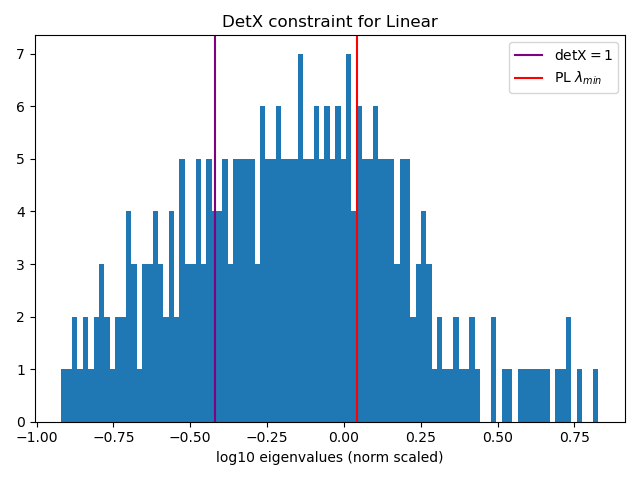
\includegraphics[width=4cm]{./img/detX_plots/LR=8/FC1/ww.layer3.detX.png}
        \label{fig:mlp3-randesd-8}
    }
    \subfigure[$LR=16\times$]{
      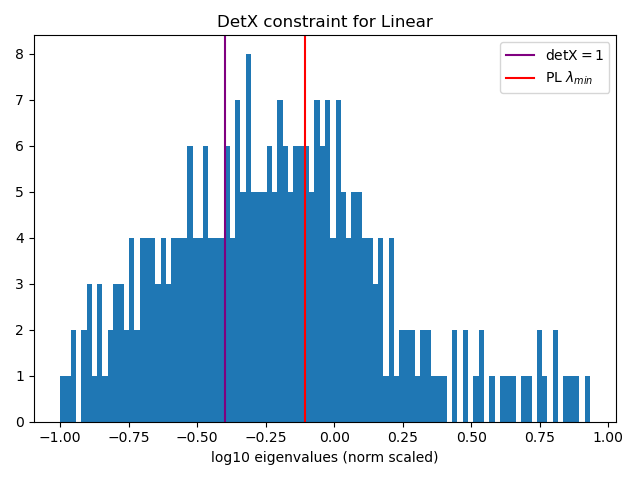
\includegraphics[width=4cm]{./img/detX_plots/LR=16/FC1/ww.layer3.detX.png}
        \label{fig:mlp3-randesd-16}
    }
    \subfigure[$LR=32\times$]{
      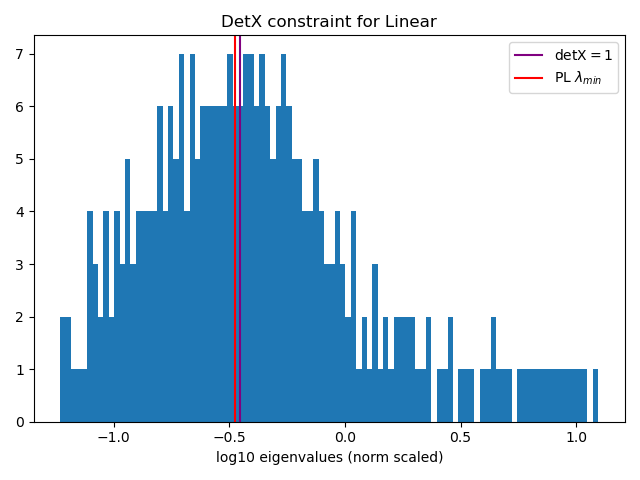
\includegraphics[width=4cm]{./img/detX_plots/LR=32/FC1/ww.layer3.detX.png}
        \label{fig:mlp3-randesd-32}
    }
    \caption{
        Log-Linear ESDs for three learning rates in the FC1 layer of MLP3. The red line shows $\LAMBDAPL$, and the 
        purple line shows $\LAMBDADETX$. Observe that the purple line is to the left of the red line, but as the LR 
        increases they move closer together. However, when LR is $32\times$, where both 
        train and test accuracy suffered (c), the red line is to the left of the purple line. This is often a signature 
        of an \OverRegularized layer, and indeed the FC1 layer in this model had $\alpha < 2$. (See Figure~\ref{fig:mlp3-alpha-fc1-by-lr} in 
        Section~\ref{sxn:empirical-test_acc}.)
        % \michael{Make the text in the fig labels large enough to read on a printed page. Also, can we make the vertical lines slightly more different colors and/or bolder.}
        %\chris{CH TODO: Hack WW to make the fig labels / ticks large enough to read here.}
    }
    \label{fig:mlp3-tracelognorm}
\end{figure}


We can compare  $\alpha$ and $\Delta \lambda_{min}$ more broadly by plotting $\Delta \lambda_{min}$ directly as a function of $\alpha$ in a single plot spanning all random seeds and learning rates or batch sizes.
This is shown in Figure~\ref{fig:mlp3-detx-gap}. 
Critical values of $\alpha=2$ and $\Delta \lambda_{min} = 0$ are shown as vertical and horizontal red lines, respectively. 
Values for various learning rates are plotted for layer FC1 
(Figure~\ref{fig:mlp3-detx-lr_search_fc1}) and FC2 (Figure~\ref{fig:mlp3-detx-lr_search_fc2}), as well as for various batch sizes in layer FC1 (Figure~\ref{fig:mlp3-detx-bs_search_fc1}) and FC2 (Figure~\ref{fig:mlp3-detx-bs_search_fc2}).

For layer FC1 (Figures~\ref{fig:mlp3-detx-lr_search_fc1} and~\ref{fig:mlp3-detx-bs_search_fc1}), in both cases we see near-linear march towards the critical tuple of $(\alpha, \Delta\lambda_{min}) = (2, 0)$.
In addition, passing this critical value coincides with diminished train and test accuracy, (recall 
Figure~\ref{fig:mlp3-accuracies}), suggesting that just as $\alpha=2$ is a threshold of over-regularization, $\LAMBDAPL < \LAMBDADETX$ may be as well. 
Since FC1 is the dominant layer, comprising roughly $8/9$ of the weights of the model, (Table~\ref{tab:mlp3},) we expect 
FC1 to most closely match the performance of the model as a whole.

For layer FC2, which comprises roughly the other $1/9$ of the models weights, there is a similar coevolution, but it is weaker. 
As learning rate or batch size exceeds their critical values, rather than going to $(2, 0)$ as in FC1, we instead see that the relationship simply breaks down, with the gap growing larger even as $\alpha$ decreases. 
Given that FC1 \emph{has} passed the critical $\alpha=2$ threshold, we conjecture that the breakdown of the relationship between $\alpha$ and $\Delta \lambda_{min}$ is due to FC1 becoming \ATypical.


\begin{figure}[t] %[h]
    \centering
    \subfigure[Layer FC1 for various learning rates]{
        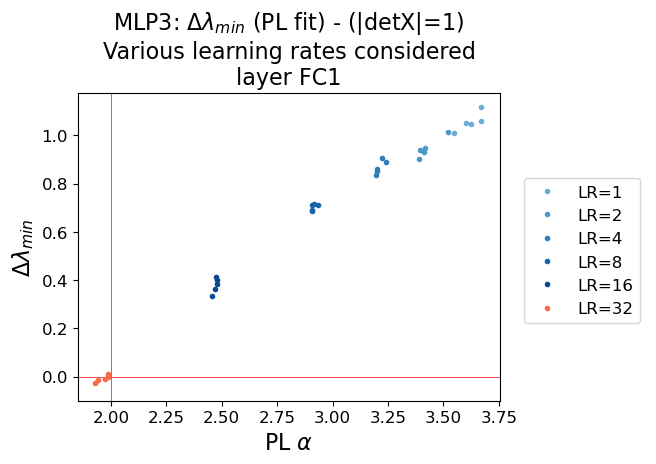
\includegraphics[width=6cm]{img/detX_plots/mlp3_detX_delta_LR_all_FC1.png}
        \label{fig:mlp3-detx-lr_search_fc1}
    }
    \subfigure[Layer FC2 for various learning rates]{
        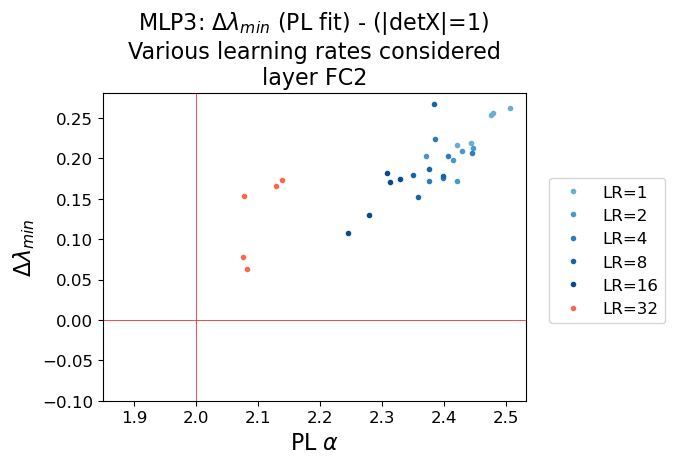
\includegraphics[width=6cm]{img/detX_plots/mlp3_detX_delta_LR_all_FC2.png}
        \label{fig:mlp3-detx-lr_search_fc2}
    }\\
    \subfigure[Layer FC1 for various batch sizes]{
        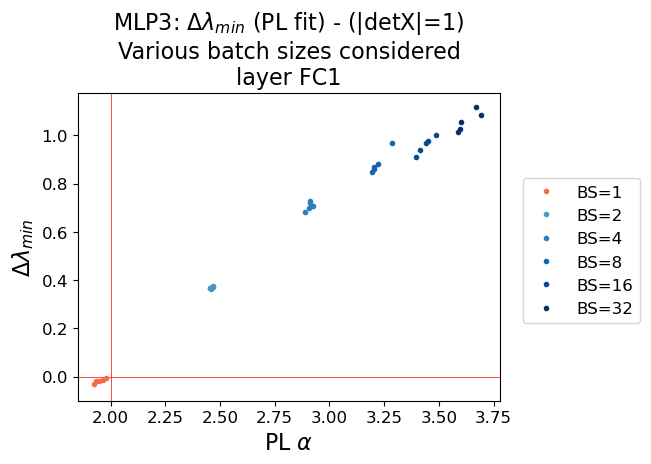
\includegraphics[width=6cm]{img/detX_plots/mlp3_detX_delta_BS_all_FC1.png}
        \label{fig:mlp3-detx-bs_search_fc1}
    }
    \subfigure[Layer FC2 for various batch sizes]{
        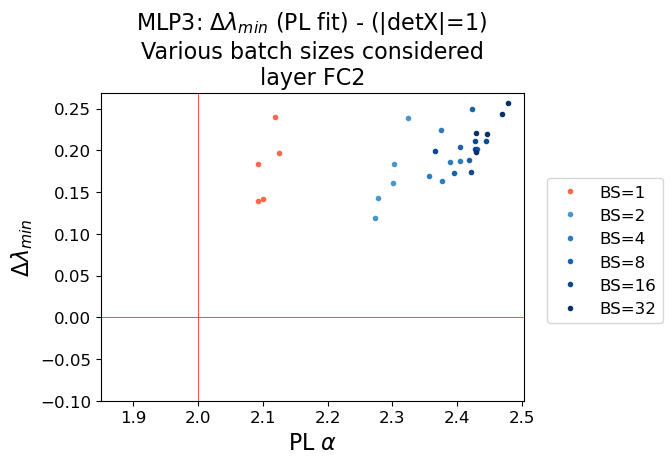
\includegraphics[width=6cm]{img/detX_plots/mlp3_detX_delta_BS_all_FC2.png}
        \label{fig:mlp3-detx-bs_search_fc2}
    }
    \caption{
            MLP3 Model: Comparison of the PL \ALPHA (x-axis), with the difference between $\LAMBDAPL$ and $\LAMBDADETX$ 
            (y-axis). The thin red lines indicate critical values of $\alpha=2$ and $\Delta \lambda_{min} = 0$. As 
            learning rate increases (a--b) or batch size decreases (c--d), we can see that in layer FC1, which dominates 
            the model, (See Table~\ref{tab:mlp3},) $\alpha$ goes to $2$, and $\Delta \lambda_{min}$ goes to $0$. Observe 
            that both critical values are crossed at the most extreme hyper-parameter selection, (red,) corresponding 
            with over-training. Layer FC2 shows a weaker tendency towards the critical values (b, d), and is disrupted 
            at the most extreme hyper-parameter values (red).
    }
 \label{fig:mlp3-detx-gap}
\end{figure}


\subsubsection{State-of-the-Art (SOTA) models}
\label{sxn:detx-sota}

Here, we consider SOTA models, 
in particular VGG pre-trained models~\cite{VGG14_TR}, the ResNet series~\cite{ResNet15_TR}, the ViT 
series~\cite{VIT20_TR}, and the DenseNet series~\cite{DenseNet17_TR}.
We show that as $\alpha$ approaches $2$, the Log-Trace Condition holds better and better, i.e., $\Delta\lambda_{min}$ 
approaches $0$.
%holds approximately for the PL portion of the tail
%even when $\alpha\gg2$ in some cases.

\begin{figure}[t] %[h]
    \centering
    \subfigure[VGG Series]{
      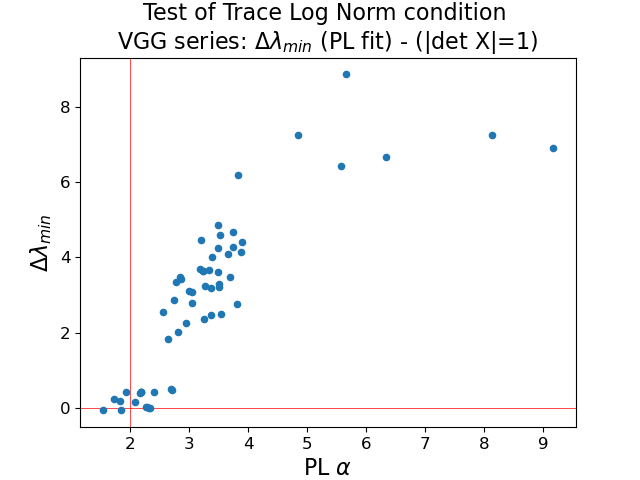
\includegraphics[width=6cm]{./img/VggTest.png}
      \label{fig:VGG_trend}
    }
    \subfigure[ResNet Series]{
      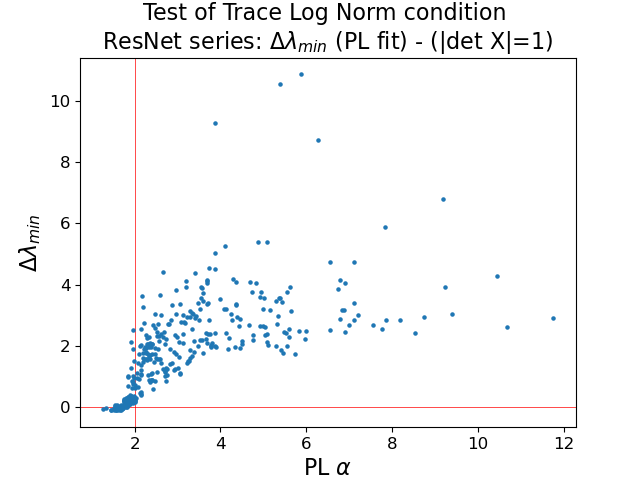
\includegraphics[width=6cm]{./img/ResNetTest.png}
      \label{fig:ResNet_trend}
    } \\
    \subfigure[ViT Series]{
      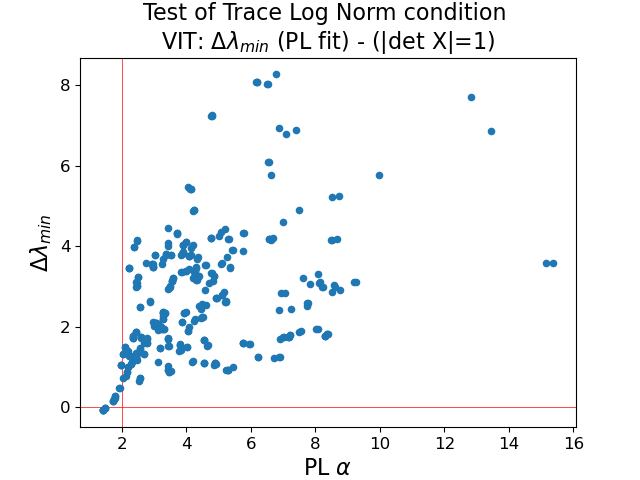
\includegraphics[width=6cm]{./img/VIT_ESD_trends.png}
      \label{fig:VIT_trend}
    }
    \subfigure[DenseNet Series]{
      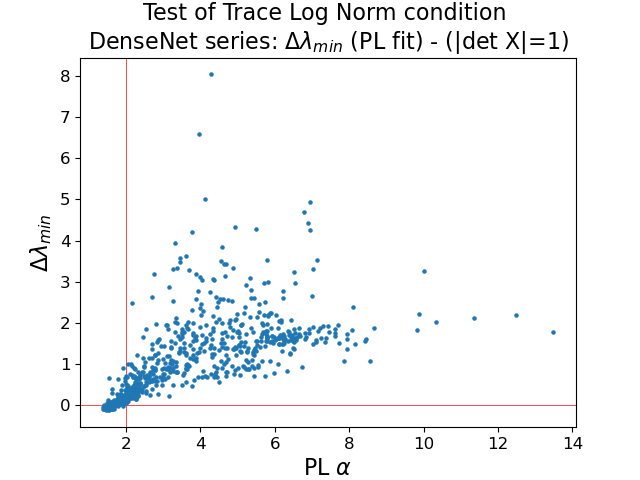
\includegraphics[width=6cm]{./img/DenseNetTest.png}
      \label{fig:DenseNet_trend}
    }
    \caption{Difference between the two $\lambda_{min}$ estimates, $\Delta\lambda_{min}$, (\EQN~\ref{eqn:D_lambda_min}), as a 
        function or $\alpha$, for linear and convolutional layers in series of VGG~\cite{VGG14_TR}, ResNet~ 
        \cite{ResNet15_TR}, ViT models~\cite{VIT20_TR} and DenseNet models~\cite{DenseNet17_TR}. Layer matrices for all 
        models in the series were pooled to create each plot. In (a), (VGG,) we see three clusters of points -- those 
        with $\Delta \lambda_{min}$ close to $0$ and $\alpha$ close to $2$, those with $\Delta \lambda_{min}$ above $2$ 
        and $\alpha > 2.5$, and those with $\Delta \lambda_{min}$ above $6$ and $\alpha > 3.5$. In (b), (ResNet,) we see 
        that in general, as $\alpha$ shrinks towards $2$, $\Delta \lambda_{min}$ tends towards $0$, overshooting 
        slightly. We also see that the difference $\Delta\lambda_{min}$ is almost always positive, with few exceptions, 
        and even the layers that do not overshoot form a kind of ``funnel shape pointing towards the critical point 
        $(2, 0)$. In (c), (ViT,) we also see the same general relationship between $\alpha$ and $\Delta \lambda_{min}$ 
        across layers of several ViT models. Observe that ViT models do not have convolutional layers, and in spite of 
        this, the overall pattern is similar. In (d), (DenseNet,) we see a similar overall trend as in (b), except that 
        $\Delta\lambda_{min}$ tends to decrease sooner, but there are also more layers with $\alpha < 2$ and 
        $\Delta\lambda_{min}$ above $0$.
    }
  \label{fig:CV_ESD_trends}
\end{figure}


Figure~\ref{fig:CV_ESD_trends} plots $\alpha$ versus the difference $\Delta\lambda_{min}$, (\EQN~\ref{eqn:D_lambda_min}).
Layer matrices from all models in each series are pooled to generate the plots.% 
\footnote{For convolutional layers, the \WW tool first computes eigenvalues for all channels-to-channels linear operators separately, and then pools them in order to compute $\alpha$, $\LAMBDAPL$ and $\LAMBDADETX$. For instance, in a $64\times 64\times 3\times 3$ weight tensor, there would be $9$ separate linear operators of $64\times 64$, giving $576$ eigenvalues, which would then be pooled to compute $\alpha$, $\LAMBDAPL$ and $\LAMBDADETX$.} 
Notice that in Figure~\ref{fig:VGG_trend} -- \ref{fig:DenseNet_trend}, $\Delta\lambda_{min}$ approaches zero as $\alpha\rightarrow 2$ from above. 
Individual points may have a large $\Delta\lambda_{min}$ for an $\alpha$ near to $2$, but the overall trend is apparent. 
The rapid decrease of $\Delta\lambda_{min}$ as $\alpha$ approaches $2$ from above, implies that the PL tail rapidly 
takes on a unit Trace-Log (if it doesnt already have it.)

As we saw in comparison of Figures~\ref{fig:mlp3-msr-results-xmin} and~\ref{fig:mlp3-msr-results-detX}, 
(Section~\ref{sxn:trunc_err_epochs},) the \TRACELOG tail is generally larger, and always has highly generalizing 
components. Thus, it is plausible that as layers reach the limit of the amount of information that can be encoded in 
them, i.e. as $\alpha$ goes to $2$, the \POWERLAW~tail expands to fill the \TRACELOG tail. This effect can be seen 
clearly in Figure~\ref{fig:CV_ESD_trends} in the condensing of the ``funnel shape.

Recall from Figure~\ref{fig:mlp3-detx-gap} that layer FC1 dominated the model, (Table~\ref{tab:mlp3},) producing a clear 
progression of $\alpha$ and $\Delta\lambda_{min}$ towards $(2, 0)$, as a function of learning rate or batch size, whereas FC2 showed a slightly less clear relationship. 
In larger models having dozens of layers, we would not expect any one layer to dominate as thoroughly.
Moreover, it is the architecture that varies between models in each series, not (necessarily) the hyperparameters, meaning that there would not be a straight linem, as in Figures~\ref{fig:mlp3-detx-lr_search_fc1} and~\ref{fig:mlp3-detx-bs_search_fc1}. 
However, with all of the layers contributing to varying degrees, we nevertheless see a clear trend in both plots of Figure~\ref{fig:CV_ESD_trends}. 
These results show how the single-layer \SETOL theory extends from the MLP3 model, which is dominated by a single layer, to larger models where many layers interact in complex ways.


\begin{figure}[t] %[h]
    \centering
    \subfigure[Falcon 7B]{
      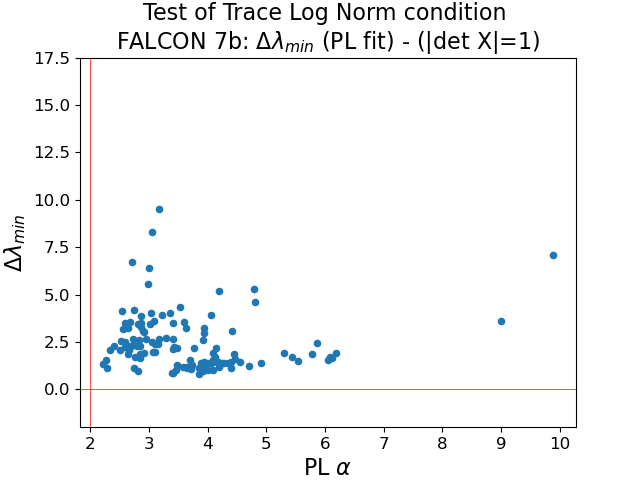
\includegraphics[width=6cm]{./img/FALCON7b_ESD_trends.png}
      \label{fig:falcon7B_trend}
    }
    \subfigure[Falcon 40B]{
      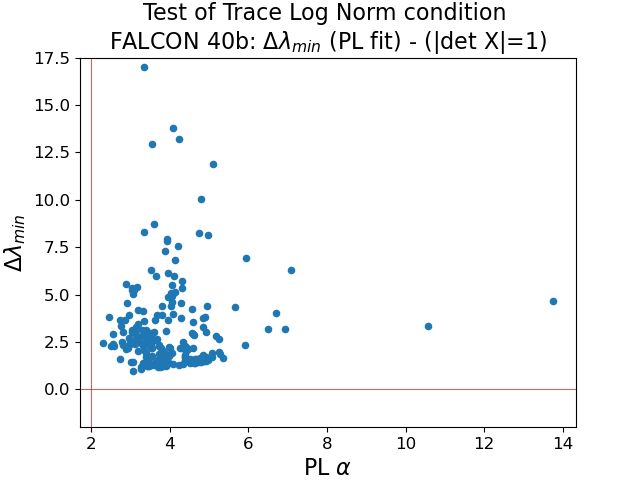
\includegraphics[width=6cm]{./img/FALCON40b_ESD_trends.png}
      \label{fig:falcon40B_trend}
    }
    \subfigure[Llama 13B]{
      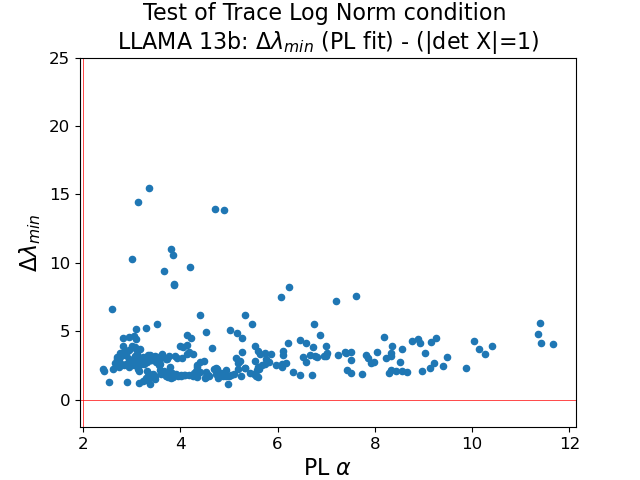
\includegraphics[width=6cm]{./img/LLAMA_13b_ESD_trends.png}
      \label{fig:llama13B_trend}
    }
    \subfigure[Llama 65B]{
      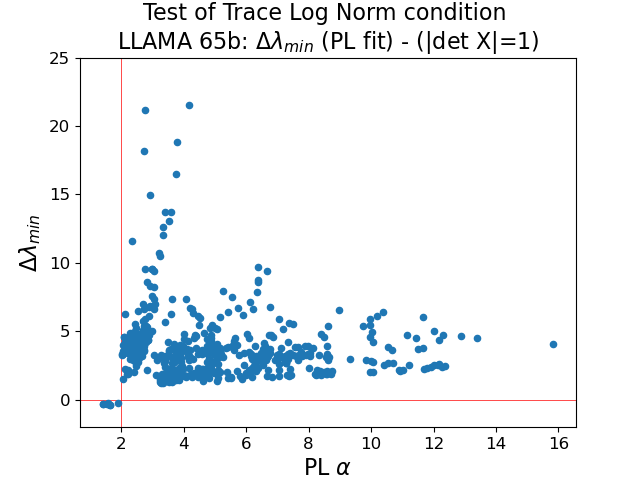
\includegraphics[width=6cm]{./img/LLAMA_65b_ESD_trends.png}
      \label{fig:llama65B_trend}
    }
    \caption{Difference between the two $\lambda_{min}$ estimates, $\Delta\lambda_{min} = \LAMBDAPL - \LAMBDADETX$, 
        as a function of $\alpha$, for all linear layers in the FALCON\cite{falcon40b}(a-b) and 
        LLAMA \cite{touvron2023_TR}(c-d) language models for varying numbers of parameters. As in Figure 
        \ref{fig:CV_ESD_trends}, we see that in recent Large Language Models, $\Delta\lambda_{min}$ remains positive, 
        except where $\alpha < 2$ (d). Otherwise, a ``funnel shape can still be seen leading towards the critical 
        point $(2, 0)$ as in Figures~\ref{fig:ResNet_trend} and~\ref{fig:VIT_trend} Observe that the x- and y-axes are 
        different between sub-figures due to the differences in scale of each model.
    }
  \label{fig:LLM_ESD_trends}
\end{figure}

The overall pattern of relationship between $\Delta\lambda_{min}$ and $\alpha$ can also be seen in 
Figure~\ref{fig:LLM_ESD_trends}, which shows plots for Large Language Models (LLMs) of the Falcon~\cite{falcon40b} and 
LLAMA~\cite{touvron2023_TR} model families, for different numbers of parameters. Observe that each 
subfigure~\ref{fig:falcon7B_trend}--\ref{fig:llama65B_trend} shows a single 
model, rather than a collection of models in a family, as in Figure~\ref{fig:CV_ESD_trends}.
The y-axis is the same between models in the same family. 
As in Figure~\ref{fig:CV_ESD_trends}, there is a general outline of a ``funnel shape pointing towards the critical 
point $(2, 0)$, with the exception that it is only reached in the case of LLAMA-65b, (Figure~\ref{fig:llama65B_trend}). 
This suggests that these LLMs are larger than they necessarily need to be, consistent with prior work~\cite{YHTx21_TR}, 
but also that they are well guarded against \OverRegularized layers beyond the critical point
($\alpha=2$ and $\Delta\lambda_{min}=0$).


